\section{Tracing}
\label{sec:tracing}
Our aim in this work was to characterize the network interaction 
between Hadoop and its related network infrastructure and the impact this 
interaction has on applications. In addition to this we aimed to 
characterize the impact of Hadoop on a datacenter network, and the 
influence of the network - its topology, protocols, and scheduling - has on the 
end-to-end application behavior. We believe this work is a good first step 
towards a better understanding of the complexity of DISC framework's interaction
with the network. In this section we discuss the components of our intial tracing
infrastructure, Section~\ref{ssec:app} disscusses application-level tracing, 
Section~\ref{ssec:low} discusses low-level tracing and lastly, 
Section~\ref{ssec:results} discussing some initial results that use our high/low-level
tracing mechanisms.

\subsection{Application-level Tracing}
\label{ssec:app}
Through the use of X-Trace~\cite{xtrace} we are able to expose causally related 
application-level events of a Hadoop job's execution. Each event that X-Trace
exposes provides us additional context about what other events came before it and
caused it to occur and similarly what events came after it. By creating X-Trace 
events for each TCP socket connect call we are able to discover the event history
for every TCP socket that is created throughout the lifetime of a job's execution.

We have augmented an X-Trace instrumented alpha version of Hadoop 2.0.4 to create 
X-Trace events for every TCP socket created. This enables us to gain a deeper insight
into every TCP socket by providing a history of events that triggered the socket and
the 5-tuple related to it (i.e. source IP/port, destination IP/port, and protocol).
Figure~\ref{fig:xtrace} is an example graphic that shows 6 causally related events that
led to a TCP socket being created. Each event box contains a unique 16 character 
identifier and a short one description of the event. Not show here for space reasons is
additional text that is displayed when a mouse is hovered over an event box. The additional
information that is displayed for the {\em SocketIOWithTimeout.connect()} event includes
the 5-tuple of the socket and a related stacktrace of events that triggered it. In addition
to the event context information an event graph is produced for each job that is submitted,
this way you can easily identify which TCP flow is associated with 

\begin{figure}
\centering
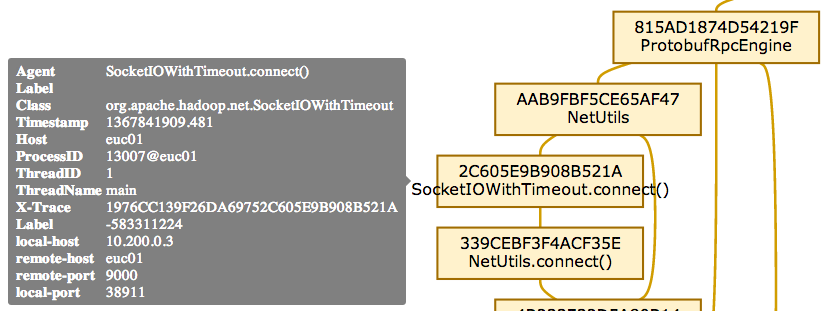
\includegraphics[width=0.7\textwidth]{figures/xtrace-example2.png}
\caption{An snippet of X-Trace events logged during a Hadoop execution.}
\label{fig:xtrace}
\end{figure}

\subsection{Lower-level Tracing}
\label{ssec:low}
Tcpdump level tracing

\subsection{Tracing Results}
\label{ssec:results}
Non-dynamic results from tracing, e.g. tput graphs, sdn tests, etc.

\begin{figure}
\centering
\begin{minipage}{.5\textwidth}
  \centering
  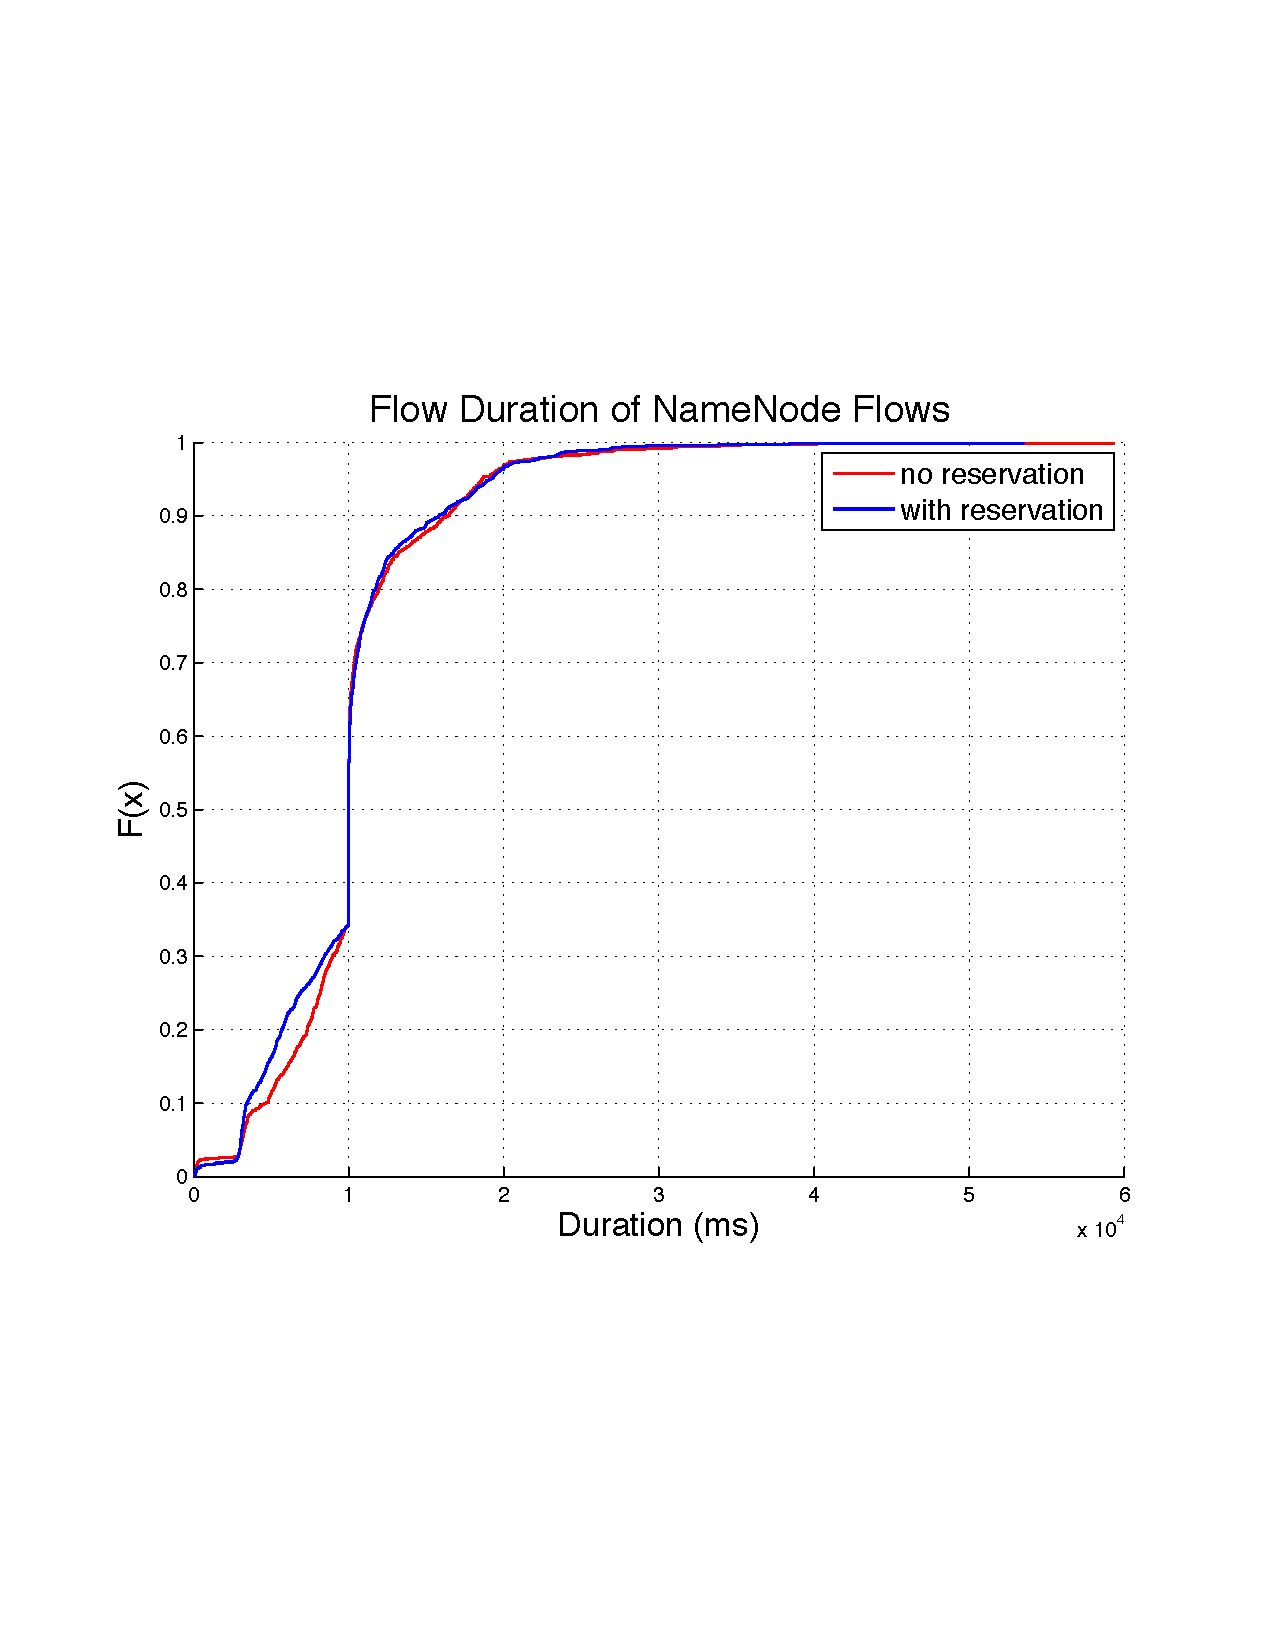
\includegraphics[width=.9\linewidth]{figures/flow_durations.pdf}
  \captionof{figure}{Duration of NameNode related flows.}
  \label{fig:duration_cdf}
\end{minipage}%
\begin{minipage}{.5\textwidth}
  \centering
  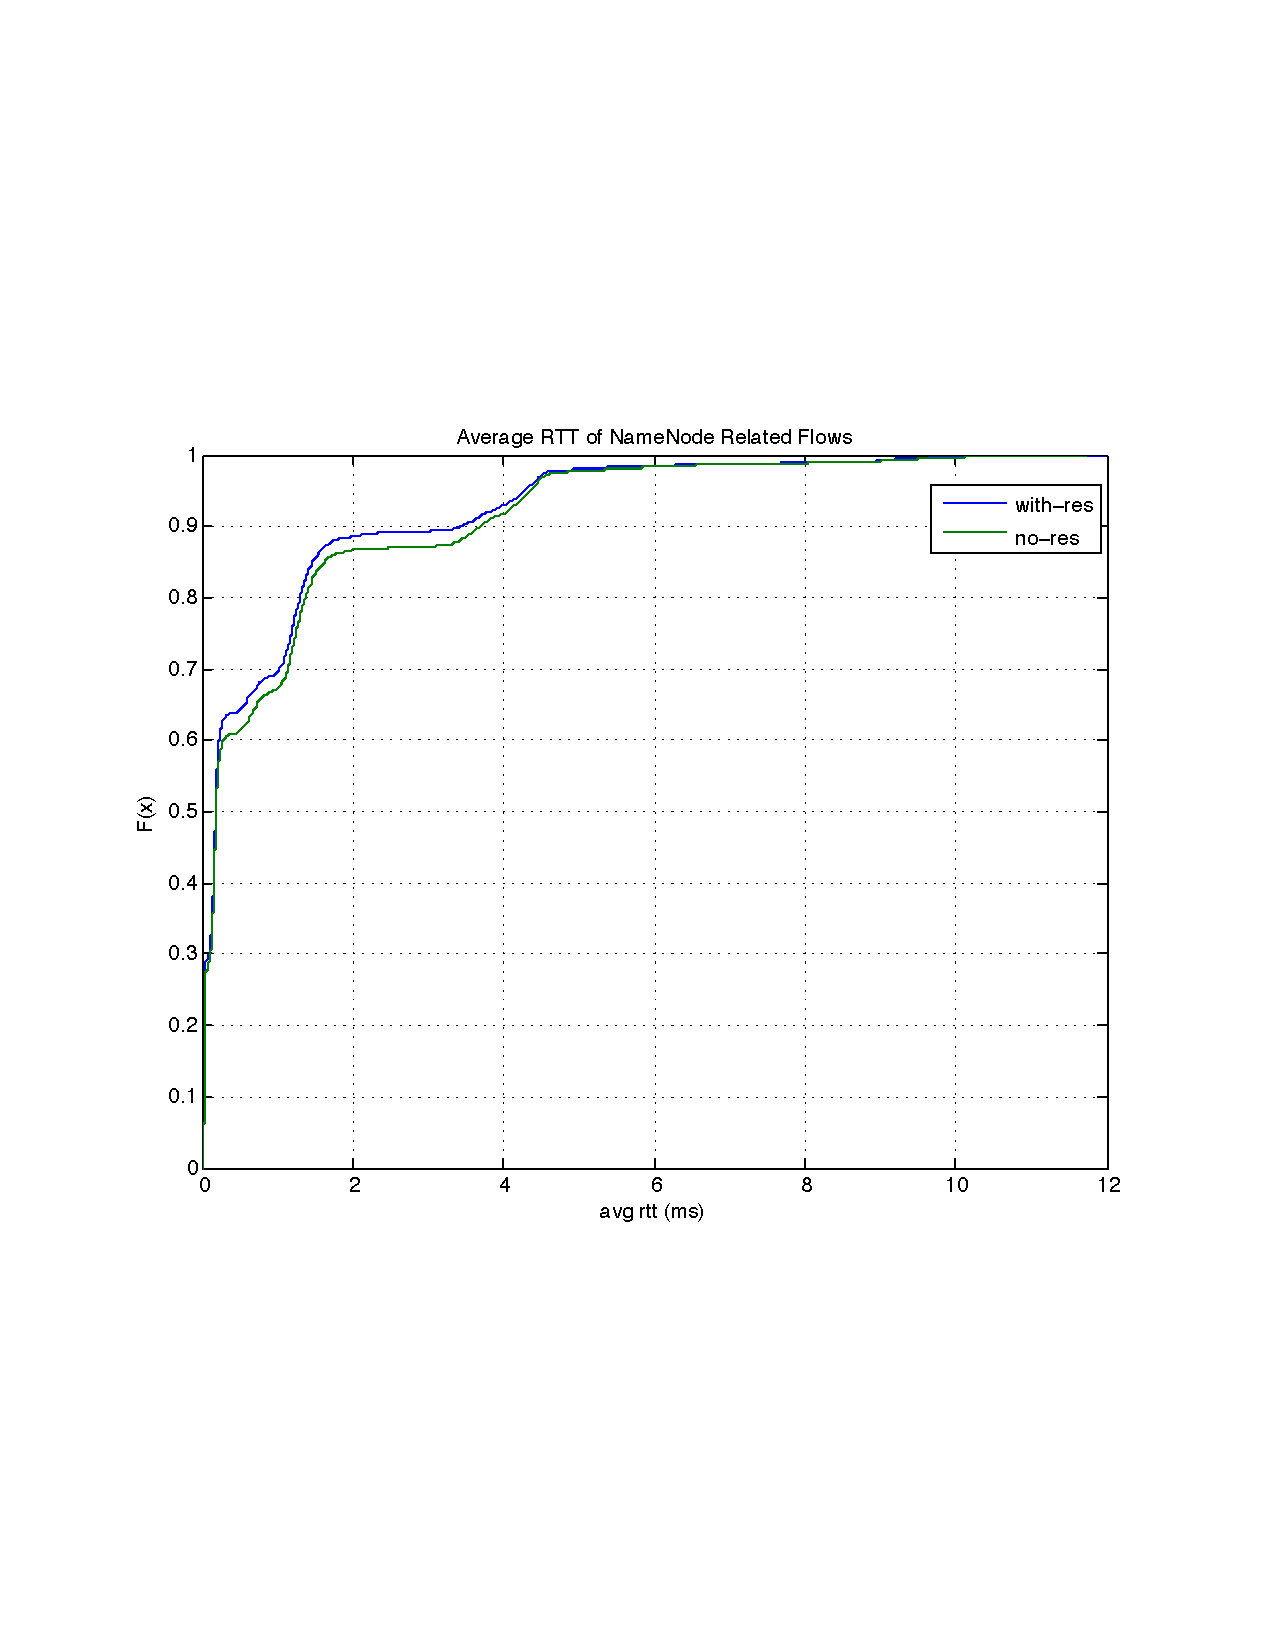
\includegraphics[width=.9\linewidth]{figures/avg_rtts_NN_flows.pdf}
  \captionof{figure}{Average RTTs for NameNode related flows.}
  \label{fig:test2}
\end{minipage}
\end{figure}

\begin{figure}
\centering
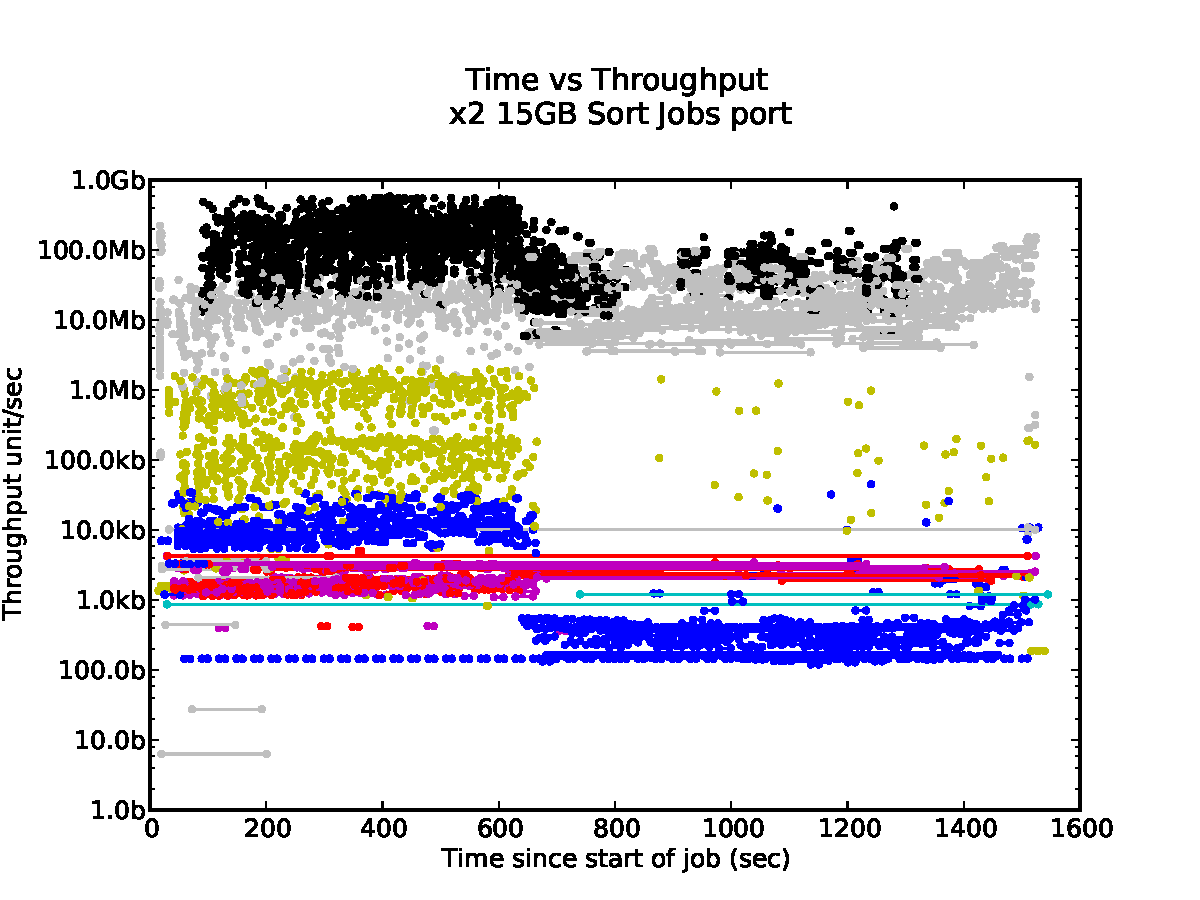
\includegraphics[width=0.7\textwidth]{figures/clock_v_throughput_port.pdf}
\caption{Average throughput of all Hadoop related flows over time.}
\label{fig:tput}
\end{figure}
